% ════════════════════════════════════════════════════════════════════════════════
\section{Architecture}
\label{sec:architecture}

\subsection{Five Processes, Two Hosts}
The system is composed of five processes spread across two hosts
(Fig.~\ref{fig:architecture}):

\begin{itemize}
  \item \textbf{UserAuthn} (\texttt{client/userauthn.py}): runs on the
    user host. Generates the PSK locally (parameter~6 of the WG config), opens the
    Noise-IK auth tunnel, drives the OAuth Device Grant, applies the WG
    config.
  \item \textbf{SrvAuthn} (\texttt{server/srvauthn.py}): runs on the
    gateway host with \texttt{network\_mode: host} so it can manage the
    in-kernel \texttt{wg0} interface. Noise-IK responder, talks to the IdP,
    generates each client's keypair, leases IPs, and registers peers.
  \item \textbf{IdP} (\texttt{idp/app.py}): Flask OAuth~2.0 server
    implementing RFC~8628~\cite{rfc8628}. Hosts the browser MFA pages,
    calls \texttt{pam\_authenticate()} via our C library.
  \item \textbf{pam\_vpnmfa.so}
    (\texttt{idp/pam\_iaa/src/pam\_vpnmfa.c}): the custom PAM module
    loaded by the IdP through the service profile
    \texttt{/etc/pam.d/iaa-vpn}.
    Decides which factors are needed and in what order
    (Section~\ref{sec:pam}).
  \item \textbf{Helpdesk} (\texttt{idp/helpdesk/app.py}): a loopback-only
    Flask app for enrolment, bound to \texttt{127.0.0.1:8081} per the
    project's instruction that the interface has no security-related
    validations (Section~\ref{sec:helpdesk}).
\end{itemize}

\begin{figure}[H]
\centering
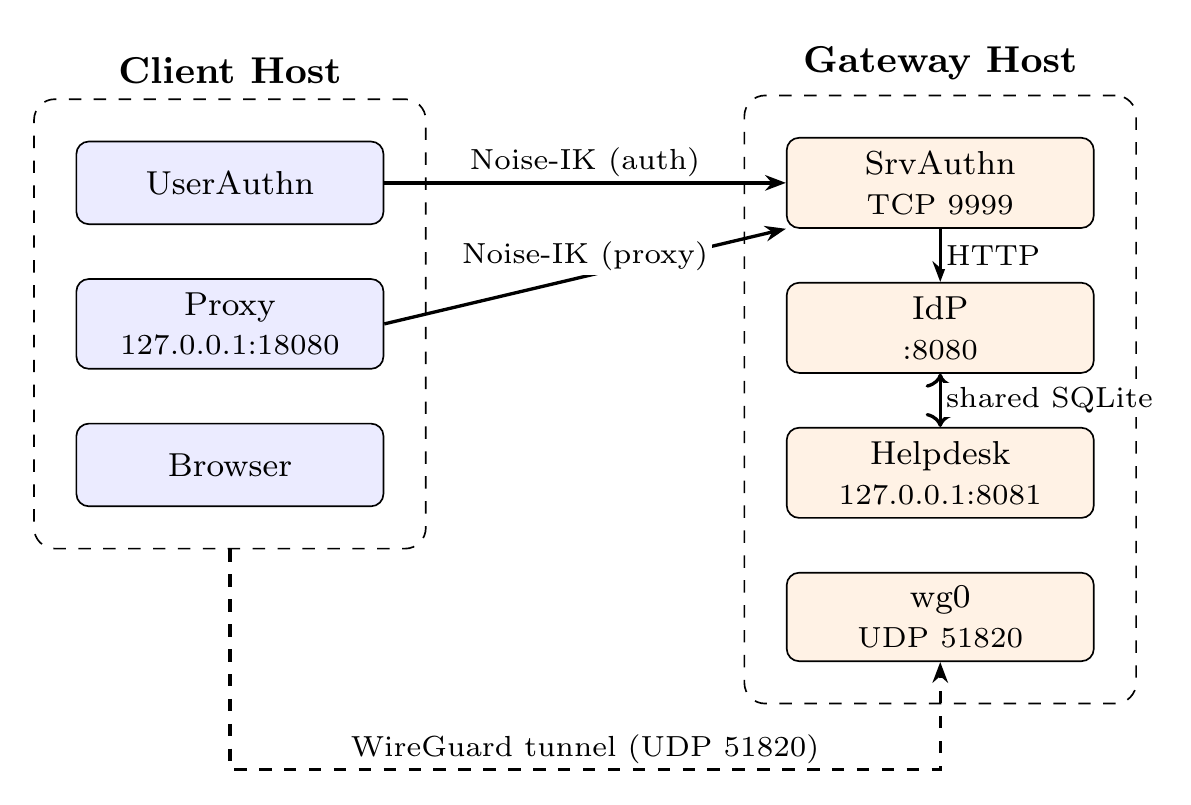
\includegraphics[width=0.9\columnwidth]{images/architecture}
\caption{Two-host deployment. Solid arrows show the authentication-phase
connections; the dashed arrow is the WireGuard data-plane tunnel that
forms after authentication.}
\label{fig:architecture}
\end{figure}

\subsection{Single Root of Trust}
\label{sec:trust}
The gateway's 32-byte Curve25519 WireGuard public key is the \emph{only}
trust anchor a client needs.
It is distributed once (in \texttt{base.conf}), and everything else
follows from it.

That single key plays two roles:

\begin{enumerate}
  \item \textbf{Noise-IK responder static key.} \texttt{SrvAuthn} loads
    \texttt{/etc/wireguard/privatekey-server} at startup and uses it as
    the Noise-IK static private key. The handshake fails with an
    AEAD-tag mismatch if a man-in-the-middle does not possess the
    matching private half.
  \item \textbf{WireGuard data-plane key.} The same private key signs
    Noise-IK handshakes for the data plane once \texttt{wg-quick up}
    runs on the client.
\end{enumerate}

The browser side is protected by the same anchor through the local HTTP
proxy (Section~\ref{sec:proxy}), so the user never has to trust a TLS
certificate.

\subsection{Deployment and Storage}
The entire stack launches with a single \texttt{docker compose up}.
Table~\ref{tab:containers} lists the four containers: three permanent
server-side processes plus an optional client used for single-machine
demos.

\begin{table}[h]
\centering
\caption{Docker containers and their network configuration.}
\label{tab:containers}
\renewcommand{\arraystretch}{1.1}
\scriptsize
\begin{tabular}{llr}
\toprule
\textbf{Container} & \textbf{Role} & \textbf{Port(s)} \\
\midrule
\texttt{vpn-idp}       & IdP, OAuth, MFA pages    & 8080 \\
\texttt{vpn-helpdesk}  & Enrolment UI (host net)  & 127.0.0.1:8081 \\
\texttt{vpn-srvauthn}  & Auth daemon + \texttt{wg0} (host net) & 9999, 51820/udp \\
\texttt{vpn-client}    & Optional demo client     & 18080 \\
\bottomrule
\end{tabular}
\end{table}

Because the three server-side processes are isolated containers, they cannot
share in-memory state.
All persistent data (user accounts, enrolled MFA credentials, active OAuth
sessions, RBA history, and WireGuard peer assignments) lives in a single
SQLite database (\texttt{/data/vpnauth.db}) that is bind-mounted into every
container that needs it.
WAL mode allows the IdP and helpdesk to read concurrently without blocking
writes from \texttt{SrvAuthn}, and the few operations that read-then-write
atomically (IP lease, nonce consumption, token redemption) use
\texttt{BEGIN IMMEDIATE} to prevent races under concurrent logins.
